\section{Introduction}
\label{chap:introduction}


Diabetes is a chronic medical condition which is estimated to affect 415 million people in the world.
 5 million deaths a year can be attributed to diabetes-related complications.
Type 2 diabetes can be prevented and reversed if diagnosed early.
We can use machine learning to predict diabetes in patients using vital 
statistics by using datasets where patients have been diagnosed. By training a neural network,
we can use it to make predictions on new patients
\\
\\
In order to run through the example below, y
ou must have installed \textcolor{blue}{Python},
setup a notebook,and create a  \textcolor{blue}{virtual environnement},and install
  all these packages:


\begin{itemize}
    \item TensorFlow
    \item Keras
    \item Seaborn
    \item pydot
    \item scikit-learn
    \item pandas
    \item Matplotlib
\end{itemize}

For this project purpose we had use 
\textbf{Anaconda },and setup a virtual environment to use a \textbf{jupiter notebook.}
\\
Learn how to how to install the prerequiste using the link below:


\url{https://towardsdatascience.com/virtual-environments-in-anaconda-jupyter}

\section{The data}
\label{chap:data}
First, we use this data set from Kaggle which tracks diabetes in Pima Native Americans.
 We use it to build a predictive model of how likely someone is to get or have diabetes given their age,
  body mass index, glucose and insulin levels, skin thickness, etc.

  \newpage

\subsection{initial observation}
\label{sec:data}
\textcolor{red}{\textbf{-Import the dataframe with pandas}}\\
We have several categories along with the outcome which is a binary classification.

\begin{figure}[htp]
    \centering
    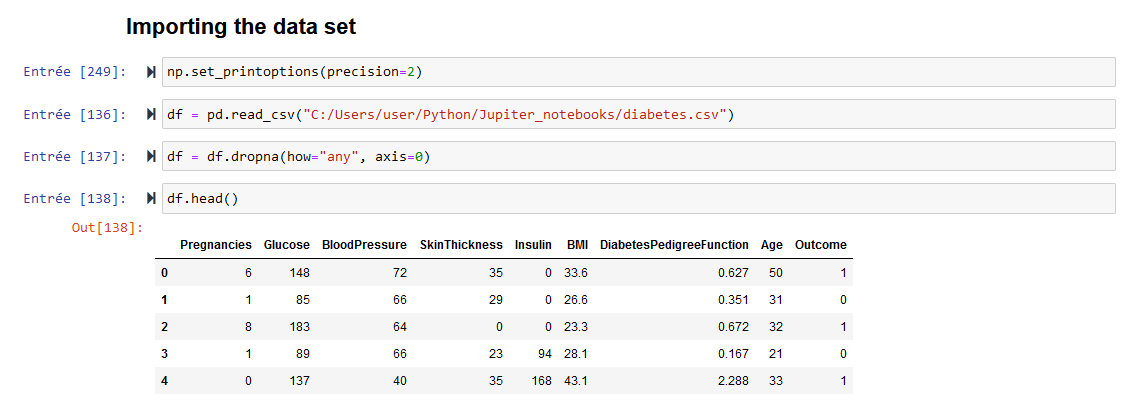
\includegraphics[width=1.5\textwidth]{images/dataframe.png}
    \caption{An exampl image}
    \label{fig:example1}
\end{figure}


\textcolor{red}{\textbf{-browse the data, listing maximum and minimum and average values}}

\begin{figure}[htp]
    \centering
    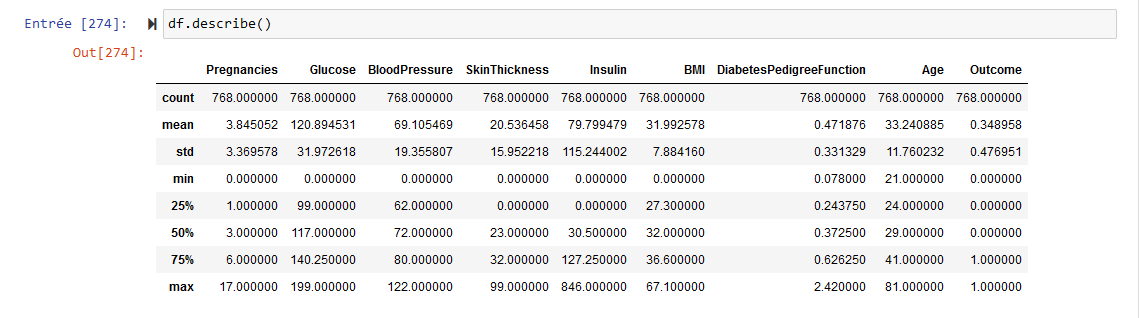
\includegraphics[width=1.3\textwidth]{images/dataframe-description.png}
    \caption{An example }
    \label{fig:example2}
\end{figure}

The data also needs to be scaled in order to allow the neural network to work effectively.
we will talk about the Data cleaning and preprocessing in the following part.

\newpage
\textcolor{red}{\textbf{-Check correlation with heatmap graph}}\\
That is not important for the final model but is useful to 
gain further insight into the data.
This is the code we used for correlation map:

\begin{lstlisting}
    import seaborn as sns
    corr = df.corr()
    sns.heatmap(corr, xticklabels=corr.columns.values,
    yticklabels=corr.columns.values)
 \end{lstlisting}

    \begin{figure}[htp]
        \centering
        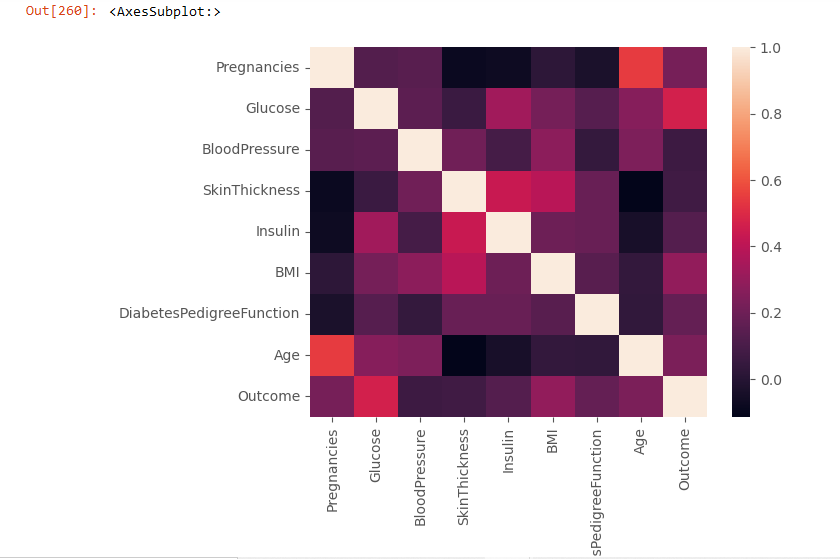
\includegraphics[width=1.1\textwidth]{images/correlation.png}
        \caption{correlation }
        \label{fig:example3}
    \end{figure}
    
   \textbf{There’s not a lot of orange squares in the chart. 
    So, you can say that no single value is 80\%. 
    likely to give you diabetes (outcome). 
    There does not seem to be much correlation between these
     individual variables. But, we will see that when taken in 
     the aggregate we can predict with almost 75\%. accuracy 
    who will develop diabetes given all of these factors together.
   }
\subsection{Data preparation}
\label{sec:data}
\textcolor{red}{Splitting the dataset into training set and test set}
\begin{lstlisting}
    labels=df['Outcome']
    features = df.iloc[:,1:8]
    from sklearn.model_selection import train_test_split
    X=features
    y=np.ravel(labels)
    X_train, X_test, y_train, y_test = train_test_split(X, y, test_size=0.33, random_state=42) 
 \end{lstlisting}

 \begin{itemize}
    \item\textbf{Outcome} is the column with the label (0 or 1). 
    \item The rest of the columns exceptthe first one are the features.
    \item We use the scikit-learn function train-test-split(X, y, testsize=0.33, randomstate=42) to split the data into training and test data sets, given 33\% of the records to the test data set. The training data set is used to train the mode, meaning find the weights and biases. The test data set is used to check its accuracy.
    \item \textbf{Label} is not an array. It is a column in a dataset. So we use the NumPy np.ravel() function to convert that to an array.
\end{itemize}
 
\textcolor{red}{Transform data in the same scale}\\
StandardScaler does this in two steps:\textcolor{blue}{\textbf{fit()}} and \textcolor{blue}{\textbf{transform()} }.\\

\begin{lstlisting}
    from sklearn.preprocessing import StandardScaler
    scaler = StandardScaler().fit(X_train)
    X_train = scaler.transform(X_train)
    X_test = scaler.transform(X_test) 
\end{lstlisting}


\section{Building the Neural Network}
\label{chap:approach}
This neural network will be built with Keras by using the Sequential class.

\begin{lstlisting}
    from keras.models import Sequential
    from keras.layers import Dense
    model = Sequential()
    model.add(Dense(7, activation='relu',input_shape=(7,)))
    model.add(Dense(7, activation='relu'))
    model.add(Dense(1, activation='sigmoid'))   
\end{lstlisting}
\subsection{Actiavtion function}
\label{sec:Actiavtion function}
  \todo[inline]{\Large Pick an activation function for each layer}
    For the first two layers we use a relu (rectified linear unit) activation function.
     That choice means nothing, as you could have picked sigmoid.
    reluI is 1 for all positive values and 0 for all negative ones
  
    \newpage

    \begin{figure}[htp]
        \centering
        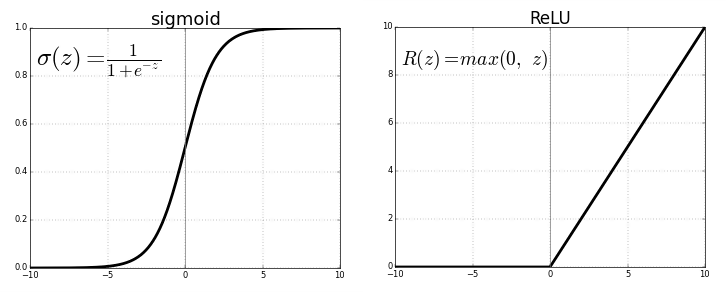
\includegraphics[width=1.1\textwidth]{images/sigmoid.png }
        \caption{sigmoid and ReLu }
        \label{fig:example4}
    \end{figure}
  
    \todo[inline]{\Large input-shape}
    we only have to give it the shape (dimensions) of the input on the first layer. 
    It’s (7,) since it’s a vector of 7 features

    \todo[inline]{\Large Dense}
    The first argument in the Dense function is the number of hidden units, 
    a parameter that you can adjust to improve the accuracy of the model

    \begin{figure}[htp]
        \centering
        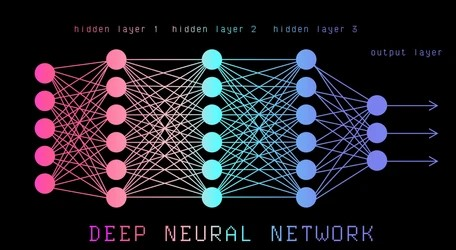
\includegraphics[width=0.9\textwidth]{images/Layers.jpg }
        \caption{Neural Network }
        \label{fig:example4}
    \end{figure}
\newpage
\subsection{Keras model fit}
\label{sec:Keras model fit}
    \begin{figure}[htp]
        \centering
        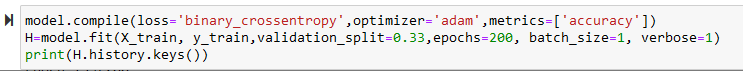
\includegraphics[width=1.3\textwidth]{images/compile.png }
        \caption{train code }
        \label{fig:example5}
    \end{figure}

    \begin{itemize}
        \item \textbf{\textcolor{red}{\Large loss:}}
        he goal of the neural network is to minimize the loss function,
        There are many functions we can use. We pick binary-crossentropy 
        because our label data is binary (1) diabetic and (0) not diabetic.

        \item \textbf{\textcolor{red}{\Large optimizer-adam:}}
        use the optimizer function adam, Adaptative moment estimation.
        It’s an algorithm designed to minimize the loss function in the quickest way possible.

        \item \textbf{\textcolor{red}{\Large Epoch:}}
        means how many times to run the model. it is an iterative process.
         You could add additional epochs, but the accuracy might not change much. 
         
        \item \textbf{\textcolor{red}{\Large batch size:}}
         means divide the input data into n batches and process each in parallel.
        \item \textbf{\textcolor{red}{\Large fit():}}
        trains the model, meaning calculates the weights, biases, number of layers, etc.
    \end{itemize}
    
    \begin{lstlisting}
        from keras.models import Sequential
        from keras.layers import Dense
        model = Sequential()
        model.add(Dense(7, activation='relu',input_shape=(7,)))
        model.add(Dense(7, activation='relu'))
        model.add(Dense(1, activation='sigmoid'))   
    \end{lstlisting}
    Above, we talked about the iterative process of solving a neural network for weights and bias.
     That’s done with epochs. Here is the output as it runs those.
     As you can see the accuracy goes up quickly then levels off.
    
     \begin{lstlisting}
        Epoch 1/30
344/344 [==============================] - 6s 16ms/step - loss: 0.5703 - accuracy: 0.7064 - val_loss: 0.5499 - val_accuracy: 0.7000
Epoch 2/30
344/344 [==============================] - 2s 5ms/step - loss: 0.4947 - accuracy: 0.7703 - val_loss: 0.5187 - val_accuracy: 0.7353
Epoch 3/30
344/344 [==============================] - 2s 5ms/step - loss: 0.4654 - accuracy: 0.7820 - val_loss: 0.5022 - val_accuracy: 0.7471    
    \end{lstlisting}
    
    \newpage
\section{Results}
\label{chap:results}

\subsection{Precision}
\label{sec:Precision}

\todo[inline]{\Large Precision}
So, our predictive model is \textbf{57\% } accurate while \textcolor{blue}{\underline{training}} and \textbf{85\% } while \textcolor{blue}{\underline {Testing}}.

\begin{figure}[htp]
    \centering
    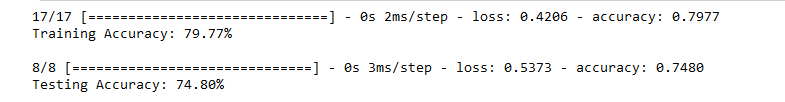
\includegraphics[width=1.3\textwidth]{images/accuracy.png}
    \caption{Neural Network }
    \label{fig:example4}
\end{figure}

\subsection{Confusion Matrix}
\label{sec:Confusion Matrix}

\todo[inline]{\Large Confusion Matrix}


\begin{figure}[htp]
    \centering
    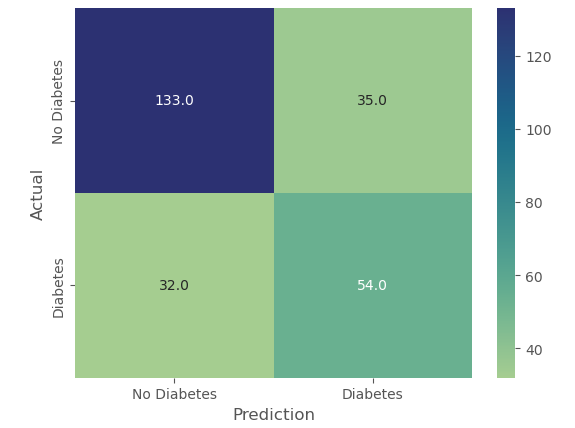
\includegraphics[width=0.7\textwidth]{images/confusion.png}
    \caption{Confusion Matrix }
    \label{fig:example5}
\end{figure}

\begin{itemize}
    \item Total in dataframe(Diabetes)=86\\
    - \textbf{wrong prediction=33}
    \item  Total in dataframe(No Diabetes)=168\\
    - \textbf{wrong prediction=40}
\end{itemize}
  

    
 A carrefull approach can permit us to say the number of (1) outcomes are thery 
 low so the model can't predict accuratly this category of persons 

 \newpage

 \subsection{classification Report}
 \label{sec:classification Report}
\todo[inline]{\Large classification Report}

Here you can see the precision is 61 for Diabetic(1) and 81 for non Diabetics(0) determiation
\begin{figure}[htp]
    \centering
    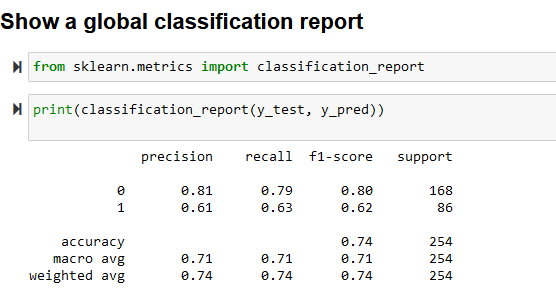
\includegraphics[width=1.2\textwidth]{images/report.png}
    \caption{Classifiaction Report }
    \label{fig:example5}
\end{figure}

\section{Discussion}
\label{chap:discussion}

Visualize Model Training History in Keras.
You can create plots from the collected history data.
he example collects the history returned from training the model and creates a chart:
         
\hspace{1cm} \textbf{\textcolor{red}{ In the same graph}}
\begin{itemize}
    \item The accuracy on the training and validation datasets over training epochs
    \item  The loss on the training and validation datasets over training epochs 
\end{itemize}
\newpage
\begin{figure}[htp]
    \centering
    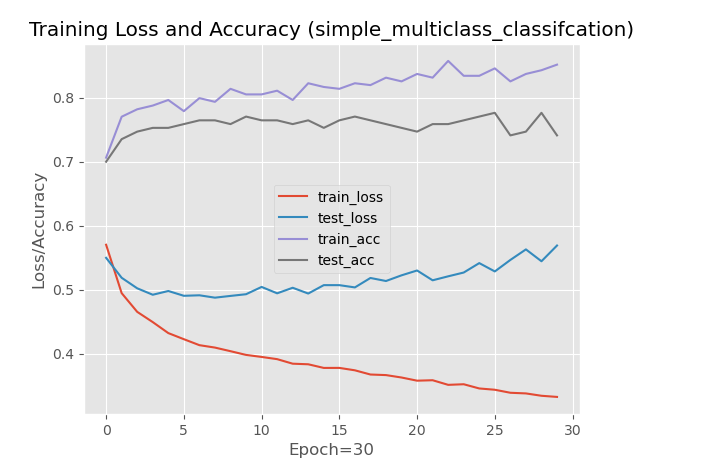
\includegraphics[width=1.2\textwidth]{images/graph.png}
    \caption{Confusion Matrix }
    \label{fig:example}
\end{figure}


\todo[inline]{
    -From the plot of the accuracy, you can see that the model could probably be trained a little more as the trend for accuracy on both datasets is still rising a little bit for the last few epochs
    }
    \todo[inline]{
    -From the plot of the loss, you can see that the model has comparable performance on both train and validation datasets (labeled test). If these parallel plots start to depart consistently, it might be a sign to stop training at an earlier epoch.
    }

\subsection{Limitations and Challenges}
\label{sec:limitation}
The test set accuracy was 79.87\% which is not too bad for
 a simple neural network, but it could certainly be improved.
  There were only 9 false positives but 22 false negatives.
   There are many improvements that need to be made to this model to 
   lower false diagnoses. This dataset only has eight categories
    which might not be enough to truly make accurate predictions.
     Feature engineering is more likely to be useful than increasing
      the complexity of this neural network.

\section{Conclusion}
\label{chap:conclusion}
It is important to note that neural networks can be more 
computationally intensive to train and may require more data and 
more time to achieve good performance, compared to some other
 classification algorithms. Additionally, they can be more difficult
  to interpret and understand, as they learn patterns in the data 
  through the weights and biases of 
the network rather than through explicit rules or decision trees.


\textbf{There are several advantages to using neural networks for classification tasks:
}
\todo[inline]{
    \\1.They are able to learn complex relationships between the input features and the target class.
    \\2.They are able to handle large amounts of data.
    \\3.They can learn from unstructured data.
    \\4.They are flexible and adaptable.
    \\5.They can be trained to perform well on a wide range of classification tasks.
}
\begin{theorem}[label={theorem:label}]{Title}
    Some text goes here!  
\end{theorem}

\newpage